\documentclass[addpoints,spanish, 12pt,a4paper]{exam}
%\documentclass[answers, spanish, 12pt,a4paper]{exam}
\printanswers
\pointpoints{punto}{puntos}
\hpword{Puntos:}
\vpword{Puntos:}
\htword{Total}
\vtword{Total}
\hsword{Resultado:}
\hqword{Ejercicio:}
\vqword{Ejercicio:}

\usepackage[utf8]{inputenc}
\usepackage[spanish]{babel}
\usepackage{eurosym}
%\usepackage[spanish,es-lcroman, es-tabla, es-noshorthands]{babel}


\usepackage[margin=1in]{geometry}
\usepackage{amsmath,amssymb}
\usepackage{multicol}
\usepackage{yhmath}

\pointsinrightmargin % Para poner las puntuaciones a la derecha. Se puede cambiar. Si se comenta, sale a la izquierda.
\extrawidth{-2.4cm} %Un poquito más de margen por si ponemos textos largos.
\marginpointname{ \emph{\points}}

\usepackage{graphicx}
\graphicspath{{../img/}} 

\newcommand{\class}{1º Bachillerato CCSS}
\newcommand{\examdate}{\today}
\newcommand{\examnum}{Examen de Álgebra}
\newcommand{\tipo}{A}


\newcommand{\timelimit}{80 minutos}

\renewcommand{\solutiontitle}{\noindent\textbf{Solución:}\enspace}


\pagestyle{head}
\firstpageheader{
\includegraphics[width=0.2\columnwidth]{header_left}}{\textbf{Departamento de Matemáticas\linebreak \class}\linebreak \examnum}{
\includegraphics[width=0.1\columnwidth]{header_right}}
\runningheader{\class}{\examnum}{Página \thepage\ of \numpages}
\runningheadrule


\begin{document}

\noindent
\begin{tabular*}{\textwidth}{l @{\extracolsep{\fill}} r @{\extracolsep{6pt}} }
\textbf{Nombre:} \makebox[3.5in]{\hrulefill} & \textbf{Fecha:}\makebox[1in]{\hrulefill} \\
 & \\
\textbf{Tiempo: \timelimit} & Tipo: \tipo 
\end{tabular*}
\rule[2ex]{\textwidth}{2pt}
Esta prueba tiene \numquestions\ ejercicios. La puntuación máxima es de \numpoints. 
La nota final de la prueba será la parte proporcional de la puntuación obtenida sobre la puntuación máxima. 

\begin{center}


\addpoints
 %\gradetable[h][questions]
	\pointtable[h][questions]
\end{center}

\noindent
\rule[2ex]{\textwidth}{2pt}

\begin{questions}

\question[1] Indica a cuáles de los conjuntos
$\mathbb{N}$, $\mathbb{Z}$, $\mathbb{Q}$, $\mathbb{R}$ pertenecen cada uno de los siguientes números:
\begin{center}
\begin{tabular}{|c |c |c |c |c|}\hline
&$\mathbb{N}$& $\mathbb{Z}$& $\mathbb{Q}$&$\mathbb{R}$\\ 
\hline
$5$&&&&\\
\hline
$-7$&&&&\\
\hline
$0,23$&&&&\\
\hline
$\sqrt{\frac{18}{2}}$&&&&\\
\hline
$-\sqrt{3}$&&&&\\
\hline
$\sqrt[3]{-5}$&&&&\\
\hline
$4,\wideparen{7}$&&&&\\
\hline
$\frac{-\pi}{2}$&&&&\\
\hline
$-\sqrt{25}$&&&&\\
\hline
$\sqrt{-4}$&&&&\\
\hline
\end{tabular}

\end{center}

\begin{solution}
\begin{tabular}{|c |c |c |c |c|}\hline
&$\mathbb{N}$& $\mathbb{Z}$& $\mathbb{Q}$&$\mathbb{R}$\\ 
\hline
$5$&X&X&X&X\\
\hline
$-7$&&X&X&X\\
\hline
$0,23$&&&X&X\\
\hline
$\sqrt{\frac{18}{2}}$&X&X&X&X\\
\hline
$-\sqrt{3}$&&&&X\\
\hline
$\sqrt[3]{-5}$&&&&X\\
\hline
$4,\wideparen{7}$&&&X&X\\
\hline
$\frac{-\pi}{2}$&&&&X\\
\hline
$-\sqrt{25}$&&X&X&X\\
\hline
$\sqrt{-4}$&&&&\\
\hline
\end{tabular}
\end{solution}

\addpoints

\question[1] Calcula:
%\noaddpoints % to omit double points count

\begin{parts}
\part $\dfrac{1}{{1 - \sqrt {2} }} - \dfrac{{3 + 3\sqrt {2} }}{{\sqrt {2} \, - 4}}$ 
\begin{solution}
$\frac{\sqrt{2}}{14} + \frac{2}{7} $ 
\end{solution}
\part $\dfrac{{\sqrt[5]{2\sqrt[4]{8}}  \cdot\sqrt {4\sqrt[3]{2}} }}{{\sqrt[12]{32} }}$
\begin{solution}
$2 \sqrt[10]{2} $
\end{solution}
\end{parts}

\question[1] Efectúa la siguiente operación, dando el resultado en notación científica y con dos cifras significativas. Da, también en notación científica, la cota del error absoluto producido en el redondeo.
$$\frac{5.12\cdot {10}^3 \cdot 4.2\cdot {10}^7}{1.8 \cdot {10}^{15}}$$
\begin{solution}
$0.000119466666666667\approx 1.2\cdot10^{-4} \to E_A < 0.05 \cdot10^{-4} = 5 \cdot10^{-6}$
\end{solution}

% \question[1] Calcula un número que restado con el doble de su raíz cuadrada nos de 15.
% \addpoints % to omit double points count
% \begin{solution}
%  	$- 2 \sqrt{x} + x - 15 = 0\to \left\{25\right\}$ 
% \end{solution}


        
\question[1] Sabiendo que log 3 = 0,477121, calcula sin usar ninguna función logarítmica de la calculadora:
         
        \begin{parts} \part  $ \log(0.003) $  \begin{solution}  $ -2.52287875 $  \end{solution} 
        % \part  $ \log(\sqrt[ 4 ]{{0.03}^3}) $  \begin{solution}  $ -1.14215906 $  \end{solution} 
        \part  $ \log(\sqrt[ 5 ]{0.81}) $  \begin{solution}  $ -0.0183029962 $  \end{solution} 
        % \part  $ \log(\frac{1}{81}) $  \begin{solution}  $ -1.90848502 $  \end{solution}
        \end{parts}
        
% \question[2] Calcula el valor de $k$ para que el resto de dividir
%   $P(x)=x^{27}-kx+3k-4$  entre  $x+1$  sea $11$    \begin{solution}  $ 4 $  \end{solution}
   
\question[2] Discute el tipo de sistema y resuelve si es posible:
  $$ \left\{\begin{matrix}2x - y + z = 6\\ 2x + 2y - 4z = 2\\ x + 3z = 2y\\ \end{matrix}\right. $$  \begin{solution}  $ \left[\begin{matrix}-1 & 2 & 1 & 6\\0 & 6 & -2 & 14\\0 & 0 & 0 & -5\end{matrix}\right] \rightarrow  \\ \left [ \right ] $  \end{solution} 

% \question[1] Discute el tipo de sistema y resuelve si es posible: $$ \left\{\begin{matrix}x + 2y - 3z = 9\\ 4x - 2y = 12\\ 4x + 3y - 6z = 24\\ \end{matrix}\right. $$  \begin{solution}  $ \left[\begin{matrix}2 & 1 & -3 & 9\\0 & 5 & -3 & 21\\0 & 0 & 0 & 0\end{matrix}\right] \rightarrow  \\ \left \{ x : \dfrac{3 z}{5} + \dfrac{21}{5}, \quad y : \dfrac{6 z}{5} + \dfrac{12}{5}\right \} $  \end{solution}


\question[2] Dos grifos abiertos de forma simultánea llenan un depósito en dos horas y cuarto. 
Sabiendo que el tiempo que tarda uno de los grifos es el cuadrado del tiempo que tarda el otro, 
calcula cuánto tarda cada grifo, por separado, en llenar el depósito.

\begin{solution}
$\left\{ \begin{matrix}\frac{1}{y} + \frac{1}{x} = \frac{4}{9} \\ y = x^{2} \\ \end{matrix}\right.$$\to \left[ \left\{ x : - \frac{3}{4}, \  y : \frac{9}{16}\right\}, \  \left\{ x : 3, \  y : 9\right\}\right]$
\end{solution}

% \question[1] En una clase los 2/3 del número de alumnas es igual a los 5/7 del número de alumnos. Si el número de
% alumnas aumenta en 26, entonces es igual al doble del número de alumnos. ¿Cuántos alumnos y alumnas
% tiene la clase?  \begin{solution}  $ \left\{\begin{matrix}\frac{2x}{3}=\frac{5y}{7}\\ x+26=2y\\ \end{matrix}\right.  \rightarrow  \\\left[\begin{matrix}- \frac{5}{7} & \frac{2}{3} & 0\\0 & \frac{13}{15} & 26\end{matrix}\right] \rightarrow  \left \{ x : 30, \quad y : 28\right \} $  \end{solution}

% \question[1] Cristina tiene 8 años más que Carlos, y hace 2 años tenía el doble de edad que él. ¿Cuántos años tiene actualmente cada uno?
% \begin{solution}
% $\left\{ \begin{matrix}y = x + 8 \\ y - 2 = 2 x - 4 \\ \end{matrix}\right.$$\to \left\{ x : 10, \  y : 18\right\}$
% \end{solution}


% \question[1] En un examen tipo test, que constaba de 40 preguntas, era obligatorio responder a todas. 
%     Cada pregunta acertada se valoró con un punto, pero cada fallo restaba medio punto. 
%     Sabiendo que la puntuación total que obtuvo Pablo fue de 32.5 puntos, 
%     ¿cuántas preguntas acertó?
% \begin{solution}
% $\left\{ \begin{matrix}x + y = 40 \\ x - \frac{y}{2} = 32.5 \\ \end{matrix}\right.$$\to \left\{ x : 35.0, \  y : 5.0\right\}$
% \end{solution}

\question[2] Resuelve las siguientes ecuaciones:
\begin{parts} \part  $ {3^{x + 1}} + {3^x} + {3^{x - 1}} = 117 $  \begin{solution}  $ \left [ 3\right ] $  \end{solution} 
\part  $ \log (x) - \log (3) = 2 $  \begin{solution}  $ \left [ 300\right ] $  \end{solution}
\end{parts}


\question[1] Resuelve el siguiente sistema :
$ \left\{\begin{matrix}\log x + \log y = 8 \\\log x - \log y = 2\end{matrix}\right. $  \begin{solution}  $ \left [ \left \{ x : 100000, \quad y : 1000\right \}\right ] $  \end{solution} 

% \question[1] Resuelve el siguiente sistema :  $ \left\{\begin{matrix}{2^{x + 2y}} = 32\\{2^{3x - 5y}} = 16\end{matrix}\right. $  \begin{solution}  $ \left [ \left \{ x : 3, \quad y : 1\right \}\right ] $  \end{solution}

% \question[1] Resuelve el siguiente sistema : $ \left\{\begin{matrix}3\log x - 2\log y = 10\\\log x + 3\log y = 7\end{matrix}\right. $  \begin{solution}  $ \left [ \left \{ x : 10000, \quad y : 10\right \}\right ] $  \end{solution}


        
\question Resuelve las siguientes inecuaciones:
 
        \begin{parts} 
        % \part[1]  $ \dfrac{{{x^3} - 5{x^2} + 2x + 8}}{x^2+1} < 0 $  \begin{solution}  $ \left(-\infty, -1\right) \cup \left(2, 4\right) $  \end{solution} 
                
        \part[1] $\dfrac{{x - 1}}{{x + 2}} \geq 0$
        \begin{solution}
        $\left(-\infty, -2\right) \cup \left[1, \infty\right)$
        \end{solution}
        % \part[1] $x^{4} + 2 x^{3} < 3 x^{2}$
        % \begin{solution}
        % $\left(-3, 0\right) \cup \left(0, 1\right)$
        % \end{solution}
        \part[1] $x^{2} - x > 2$
        \begin{solution}
        $\left(-\infty, -1\right) \cup \left(2, \infty\right)$
        \end{solution}
        
        % \part[1]  $2 < \left|{x - 1}\right|$  \begin{solution}  $ \left(-\infty < x \wedge x < -1\right) \vee \left(3 < x \wedge x < \infty\right) $  \end{solution} 
        
        \part[1]  $ \left|{x - 1}\right| > 2$  \begin{solution}  $ \left(-\infty < x \wedge x < -1\right) \vee \left(3 < x \wedge x < \infty\right) $  \end{solution} 
        
        % \part[1] $x^{4} + 2 x^{3} < 3 x^{2}$
        % \begin{solution}
        % $\left(-3, 0\right) \cup \left(0, 1\right)$
        % \end{solution}
        \end{parts}

        % \question Resuelve, justificadamente, los siguientes sistemas de inecuaciones:
        % \begin{parts} 
        %  \part[1]  $$ \left\{\begin{matrix}{( {x - 1} )^2} - {( {x + 3} )^2} \leq 0\\x - 3( {x - 1} ) \geq 3 \end{matrix}\right. $$  
        %  \begin{solution}  $ \left[-1, 0\right] $  \end{solution}
        %  \part[2]  $$ \left\{\begin{matrix}x \geq 0 \\0 \leq y \leq 3\\x - 2y \leq 10\\x + y \geq 10\\\end{matrix}\right. $$  \begin{solution}   \\ 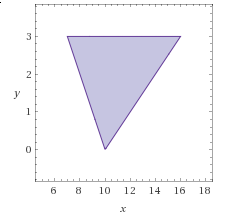
\includegraphics[width=1\columnwidth]{si5}   \end{solution}  
        % \end{parts}




\addpoints

\end{questions}

\end{document}
\grid
